\documentclass{article}

\usepackage[final]{neurips_2020}

\usepackage[utf8]{inputenc}
\usepackage[T1]{fontenc}
\usepackage{hyperref}
\usepackage{url}
\usepackage{booktabs}
\usepackage{amsfonts}
\usepackage{nicefrac}
\usepackage{microtype}
\usepackage{graphicx}
\usepackage{xcolor}
\usepackage{amsmath}
\usepackage{tikz}
\usetikzlibrary{arrows.meta, positioning, shapes.geometric}
\usetikzlibrary{patterns}
\usepackage{float}
\usepackage{CJKutf8}

\newcommand{\note}[1]{\textcolor{blue}{{#1}}}

\title{
  Retriever-Aware Selective Query Rewriting
  
  for Korean RAG \\
  \vspace{1em}
  \small{\normalfont Korea University COSE461 Final Project}
}

\author{
   GyeongLim Kang \\
   Department of Computer Science \\
   Team 8 \\
   2021320112
  % Examples of more authors
   \And
   Seunghwan An \\
   Department of Computer Science \\
   Team 8 \\
   2021320161
}

\begin{document}

\maketitle

\begin{abstract}
Query rewriting can improve retrieval in Retrieval-Augmented Generation (RAG), but unnecessary rewriting may degrade queries that already retrieve relevant evidence well. This work investigates when query rewriting is beneficial in Korean RAG and proposes a retriever-aware selective rewriting framework. The proposed method uses a confidence gate to decide whether intervention is needed and a selective policy to choose between preserving the original query and applying a rewrite strategy. Experiments across Korean QA datasets show that rewriting affects retrievers differently: BM25 and hybrid retrieval benefit from selective rewriting, whereas dense retrieval requires more conservative treatment. In an offline oracle-feature analysis, the proposed policy improves Hybrid Recall@10 from 0.1467 to 0.2400 on held-out challenging cases, while a score-based gate limits unnecessary intervention on general queries. These results suggest that query rewriting should be applied selectively according to retriever behavior rather than used unconditionally.
\end{abstract}

\section{Introduction}

Retrieval-Augmented Generation (RAG) relies on retrieving relevant external 
evidence to produce grounded answers~\cite{lewis2020rag}. However, natural-language 
questions are not always effective retrieval queries: they may omit key terms or 
use expressions that differ from the supporting passage. Query rewriting addresses 
this mismatch by reformulating questions into retrieval-friendly queries
~\cite{ma2023rewrite,chan2024rqrag}.

Recent work optimizes query rewriting using retrieval-oriented feedback, showing 
that a useful rewrite should improve retrieval rather than merely sound fluent
~\cite{wu2022conqrr,mao2024rafe,zhu2025maferw}. However, whether rewriting 
should be applied at all remains less explored. This matters because rewriting an 
already effective query can introduce irrelevant terms or semantic drift. Moreover, 
rewriting effects can differ by retriever: lexical retrieval may benefit from 
additional keywords, whereas dense retrieval may be harmed by unnecessary 
reformulation, consistent with recent retriever-specific rewriting findings
~\cite{cha2025rlqr}.

We therefore propose a retriever-aware selective query rewriting framework for 
Korean RAG. Our method treats preserving the original query as an explicit action 
alongside four rewrite strategies: keyword, expanded, structured, and LLM-based 
rewriting. It first applies a confidence gate to determine whether intervention is 
needed, and then uses a reward-validated policy to select an appropriate action for 
the target retriever. We evaluate the label-guided component offline with manual
failure labels and logged gold-rank buckets, leaving fully automatic feature
prediction for future work.

We evaluate the framework with BM25, dense, and hybrid retrievers on Korean QA data 
and a manually annotated challenging-case set. Our results show that selective 
rewriting benefits BM25 and hybrid retrieval, while dense retrieval requires more 
conservative intervention. In our offline oracle-feature analysis, our policy improves Hybrid Recall@10 from 
$0.1467$ to $0.2400$ on held-out challenging cases, supporting selective rather than 
unconditional query rewriting.

Our main contributions are as follows:
\begin{itemize}
    \item We formulate query rewriting as a selective decision problem that 
    explicitly includes preserving the original query.
    \item We propose a two-stage framework combining a confidence gate with a 
    retriever-aware selective policy.
    \item We analyze retriever-specific rewrite behavior using a manually annotated 
    Korean challenging-case set.
\end{itemize}

\section{Related Work}

We organize prior work into query rewriting frameworks, feedback-guided
rewriting, and adaptive retriever-specific rewriting.

\subsection{Query Rewriting for Retrieval-Augmented Generation}

Rewrite-Retrieve-Read~\cite{ma2023rewrite} inserts a rewriting module before
retrieval, and RQ-RAG~\cite{chan2024rqrag} extends rewriting into multiple
refinement actions such as rewriting, decomposition, and disambiguation. Our
action space follows this view that different query problems may require
different refinement operations. However, these frameworks still emphasize how
to transform a query once rewriting is chosen, and usually evaluate rewriting as
a generally useful preprocessing step. We instead treat \texttt{original} as a
first-class action, so the policy can decide not to rewrite at all when the
original query is already effective.

\subsection{Feedback-Guided and Reinforcement Learning-Based Rewriting}

Recent work evaluates rewrites by retrieval utility rather than fluency.
CONQRR~\cite{wu2022conqrr} optimizes conversational rewriting with retrieval
rewards, while RaFe~\cite{mao2024rafe} uses reranker-based ranking feedback to
train a generative rewriter. MaFeRw~\cite{zhu2025maferw} further combines
ranking, document similarity, and answer-quality signals. These works motivate
our reward-based evaluation and our use of retrieval and answer-support metrics
rather than surface fluency. In particular, they support the view that a rewrite
is useful only if it improves downstream evidence retrieval. The main difference
is that they primarily improve a rewriter; we instead select whether to keep the
original query or apply one of several rewrite strategies.

\subsection{Adaptive and Retriever-Specific Rewriting}

RL-QR~\cite{cha2025rlqr} shows that rewriting effects depend on the retriever,
with stronger gains for lexical retrieval than for semantic or hybrid retrieval.
Q-PRM~\cite{wang2024qprm} similarly argues that query refinement can be excessive
or insufficient depending on query complexity. These findings match our
observation that lexical retrieval can benefit from added terms, whereas dense
retrieval can be hurt by unnecessary reformulation. They motivate our
retriever-aware gate and selective policy. Rather than assuming a single rewrite
policy transfers across retrieval paradigms, we explicitly condition the
rewriting decision on retriever behavior and decide when rewriting is likely to
help.

\section{Approach}

\subsection{Problem Setup and Action Space}
\label{sec:setup}

Let $q$ be an input question, $\mathcal{D}$ a document collection, and
$r \in \{\textsc{bm25}, \textsc{dense}, \textsc{hybrid}\}$ a retriever. A
\emph{query action} $a$ maps $q$ to a transformed query $q' = a(q)$, and the
retriever returns a ranked list $\pi_r(q', \mathcal{D})$. We evaluate retrieval
with $\mathrm{Recall@10}$ and $\mathrm{MRR}$, measure answer support with
$\mathrm{AnswerSupport\ F1}$, and summarize them with a composite scalar
$\mathrm{Reward}$ (Section~\ref{sec:eval}).

We define a fixed, interpretable action space
\begin{equation}
\mathcal{A} = \{\,
\texttt{original},\;
\texttt{keyword},\;
\texttt{expanded},\;
\texttt{structured},\;
\texttt{llm}
\,\},
\end{equation}
where \texttt{original} preserves the user query ($a(q)=q$), \texttt{keyword}
compresses it to core terms, \texttt{expanded} adds related or missing terms,
\texttt{structured} reorganizes it into a retrieval-friendly form, and
\texttt{llm} produces a fluent retrieval-oriented rewrite. \textbf{Including
\texttt{original} as an explicit action---so the policy can choose not to
rewrite---is one of our original contributions}; prior rewriting
work~\cite{ma2023rewrite, mao2024rafe} implicitly assumes some transformation is
always applied. The full inference pipeline is shown in
Figure~\ref{fig:pipeline}.

\begin{figure}[ht]
\centering
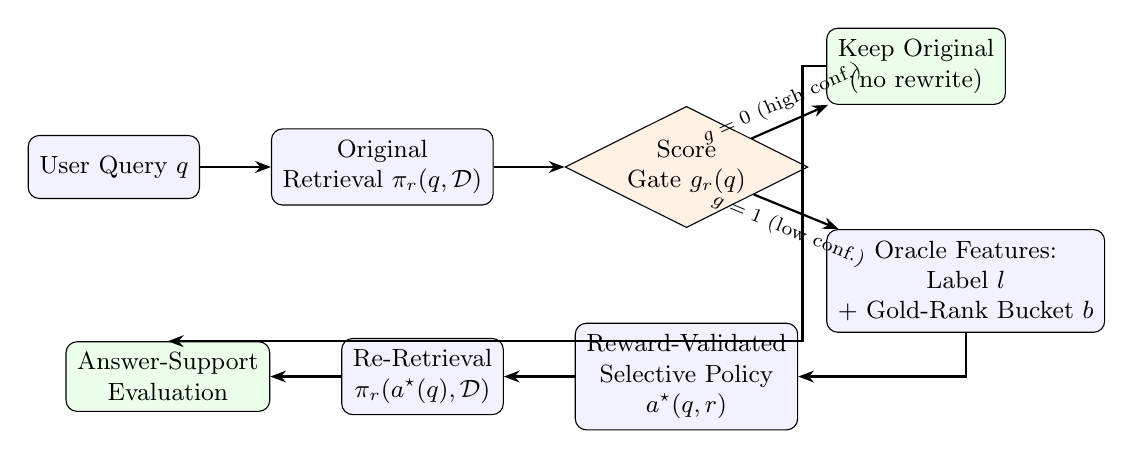
\begin{tikzpicture}[
  font=\small,
  box/.style={draw, rounded corners, align=center, minimum height=8mm,
              inner sep=4pt, fill=blue!5},
  dec/.style={draw, diamond, aspect=2, align=center, inner sep=1pt,
              fill=orange!10},
  term/.style={draw, rounded corners, align=center, minimum height=8mm,
               inner sep=4pt, fill=green!8},
  arr/.style={-{Stealth[length=2mm]}, thick},
  node distance=6mm and 9mm
]
\node[box] (q) {User Query $q$};
\node[box, right=of q] (ret) {Original\\Retrieval $\pi_r(q,\mathcal{D})$};
\node[dec, right=of ret] (gate) {Score\\Gate $g_r(q)$};
\node[term, above right=4mm and 10mm of gate] (keep) {Keep Original\\(no rewrite)};
\node[box, below right=4mm and 10mm of gate] (hard) {Oracle Features:\\Label $l$\\+ Gold-Rank Bucket $b$};
\node[box, below=12mm of gate] (pol) {Reward-Validated\\Selective Policy\\$a^\star(q,r)$};
\node[box, left=of pol] (rerank) {Re-Retrieval\\$\pi_r(a^\star(q),\mathcal{D})$};
\node[term, left=of rerank] (ans) {Answer-Support\\Evaluation};

\draw[arr] (q) -- (ret);
\draw[arr] (ret) -- (gate);
\draw[arr] (gate) -- node[above, sloped, font=\scriptsize] {$g=0$ (high conf.)} (keep);
\draw[arr] (gate) -- node[below, sloped, font=\scriptsize] {$g=1$ (low conf.)} (hard);
\draw[arr] (hard) |- (pol);
\draw[arr] (pol) -- (rerank);
\draw[arr] (rerank) -- (ans);
\draw[arr] (keep.west) -- ++(-0.3,0) |- (ans.north);
\end{tikzpicture}
\caption{Selective rewriting pipeline. A score gate decides whether to
intervene; low-confidence queries are routed to a retriever-aware policy that
may rewrite or keep the original query.}
\label{fig:pipeline}
\end{figure}

\subsection{Retrievers and Baselines}
\label{sec:retrievers}

We build on three standard retrievers, none of which is a contribution of this
work. \textbf{BM25} is a sparse lexical retriever, implemented with
Pyserini~\cite{lin2021pyserini}. \textbf{Dense} retrieval uses the
\texttt{intfloat/multilingual-e5-base} bi-encoder~\cite{wang2024me5} served
through Sentence-Transformers~\cite{reimers2019sbert}. \textbf{Hybrid} retrieval
linearly fuses the two normalized scores,
\begin{equation}
S_{\text{hybrid}} = \alpha\, S_{\textsc{bm25}} + (1-\alpha)\, S_{\textsc{dense}},
\label{eq:hybrid}
\end{equation}
with the interpolation weight $\alpha$ selected on a held-out validation split
by an MRR-based sweep, yielding $\alpha = 0.1$ (i.e.\ a dense-dominant fusion
with a small lexical contribution).

These retrievers also define our \emph{baselines} for the selection problem:
\textbf{original-only} (always \texttt{original}; the no-rewrite lower anchor),
\textbf{always-LLM} (always \texttt{llm}; unconditional rewriting, the implicit
strategy of prior work and the one our thesis argues against), and
\textbf{oracle-best} (per-query best \emph{observed} action; an upper bound that
is not deployable).

\subsection{Challenging-Case Set Construction}
\label{sec:hardcase}

\textbf{(Original contribution.)}
To study \emph{when} rewriting helps across retrieval paradigms, we construct a
Korean RAG challenging-case set by sampling queries for which at least one of
BM25, Dense, or Hybrid retrieval fails to place the gold passage in the top-10
under the original query. Using fixed dataset quotas and seed $42$, we collect
$1{,}000$ cases from KorQuAD~1.0~\cite{lim2019korquad} ($200$),
KLUE-MRC~\cite{park2021klue} ($350$), and
KorQuAD~2.0~\cite{kim2019korquad2} ($450$), evaluate them across BM25, Dense,
and Hybrid, and split them into $700$ training and $300$ held-out test cases.

Each query receives one dominant manual failure label among seven categories:
\texttt{lexical\_mismatch} (310), \texttt{missing\_key\_term} (275),
\texttt{numeric\_temporal\_mismatch} (218), \texttt{entity\_mismatch} (98),
\texttt{ambiguous} (59), \texttt{context\_boundary\_issue} (39), and
\texttt{semantic\_mismatch} (1). Sparse categories are merged into broader
groups for policy estimation; this simplifies estimation but cannot represent
different failure reasons for the same query across retrievers.

\paragraph{Label refinement.}
To reduce sparsity, we deterministically merge rare or overlapping failure
labels: numeric or temporal cases are grouped as
\texttt{numeric\_temporal\_mismatch}, rare \texttt{semantic\_mismatch} cases are
merged into \texttt{lexical\_mismatch}, short \texttt{ambiguous} queries are
treated as \texttt{missing\_key\_term}, and at most one secondary diagnostic
suffix is retained.

\subsection{Reward-Validated Label-Guided Selective Policy}
\label{sec:policy}

\textbf{(Main methodological contribution.)} Our policy is \emph{not} a
parameterized RL model; it is a reward-validated, label-guided action selector
designed for robustness on a small, noisily labeled challenging-case set. The
decision conditions on three discrete factors: the retriever $r$, the refined label
$l = l(q)$, and an \emph{original-rank bucket} $b(q)\in\{\texttt{failed},
\texttt{rank\_1}, \texttt{rank\_2\_5}, \texttt{rank\_6\_10}\}$ that captures how
well the original query already retrieved.

This selective policy is evaluated in an oracle-feature setting: the refined
failure label and the original gold-rank bucket are taken from manual annotation
and logged retrieval results. It therefore measures the potential benefit of
failure-aware action selection rather than a fully automatic deployment policy.
Replacing these oracle features with inference-time signals is left for future
work.

\paragraph{Training: utility estimation.}
On the training split, we estimate the mean utility of each action for each
$(r,l,b)$ context,
\begin{equation}
\widehat{U}(a \mid r, l, b) =
\frac{1}{|\mathcal{D}_{r,l,b}|}
\sum_{q \in \mathcal{D}_{r,l,b}} \mathrm{Reward}_r\big(a(q)\big),
\label{eq:utility}
\end{equation}
where $\mathcal{D}_{r,l,b}$ is the set of training challenging cases in that context.
The test split is never used in Eq.~\eqref{eq:utility}, preventing leakage.

\paragraph{Recovery utility for retrieval failures.}
For queries with original-retrieval failure, the primary objective is to recover
the gold passage into the top-10.
To capture this, we define a \emph{recovery utility} that measures the change
each action produces relative to the original query:
\begin{equation}
U_{\text{rec}}(a \mid q) =
\Delta\mathrm{Recall@10}
+ 0.25\,\Delta\mathrm{MRR}
+ 0.10\,\Delta\mathrm{AnswerSupport\ F1}
+ 0.05\,\Delta\mathrm{Reward},
\label{eq:recovery}
\end{equation}
where each $\Delta(\cdot) = (\cdot)_{a(q)} - (\cdot)_{q}$ is the change relative
to the original query. The dominant weight on $\Delta\mathrm{Recall@10}$ encodes
that recovering the gold passage into the top-10 is the primary objective for
retriever-specific failures, with ranking, answer, and overall-utility improvements serving as
secondary tie-breakers. Although Reward already includes retrieval and
answer-support components, its small coefficient in $U_{\text{rec}}$ is used
only as a penalty-aware tie-breaker. Equation~\eqref{eq:recovery} is our own
design.

\paragraph{Inference: conservative override.}
A retriever-tuned base action $a_{\text{base}}$ is proposed first, using a
retriever-appropriate objective: BM25 optimizes MRR improvement (lexical
rewrites tend to raise the gold passage's rank), Dense optimizes overall reward
improvement (to penalize semantic drift), and Hybrid optimizes the recovery
utility $U_{\text{rec}}$ of Eq.~\eqref{eq:recovery} (to prioritize converting
failures into top-10 hits). The label-guided action
$a_{\text{label}} = \arg\max_{a}\widehat{U}(a \mid r,l,b)$ overrides the base
action only when its estimated utility advantage exceeds a margin $\tau = 0.02$:
\begin{equation}
a^{\star}(q, r) =
\begin{cases}
a_{\text{label}}, &
\text{if } \widehat{U}(a_{\text{label}} \mid r,l,b)
            - \widehat{U}(a_{\text{base}} \mid r,l,b) \ge \tau, \\[4pt]
a_{\text{base}}, & \text{otherwise.}
\end{cases}
\label{eq:override}
\end{equation}
Small utility differences---likely annotation noise---thus default to the safer
base action, while label guidance intervenes only with clear training-set
evidence. The conditioning on $b(q)$ further suppresses needless rewriting: a
\texttt{rank\_1} query is already well served and is typically left unchanged.

\subsection{Score-Gated Rewriting for General Queries}
\label{sec:gate}

For arbitrary queries, a score-based gate $g_r(q)$ decides whether intervention
is needed. Since manual failure labels are unavailable outside the annotated
set, routed queries use a label-free action scorer:
\begin{equation}
a_{\mathrm{gen}}^\star(q,r)
=
\arg\max_{a \in \mathcal{A}} f_r(q,a),
\end{equation}
where $f_r$ is trained on challenging-case training data to predict recovery
utility from retriever, query, action, and logged gold-rank-derived features.
The final action is
\begin{equation}
a_{\text{final}}(q, r) =
\begin{cases}
\texttt{original}, & g_r(q)=0, \\
a_{\mathrm{gen}}^\star(q,r), & g_r(q)=1.
\end{cases}
\label{eq:gate}
\end{equation}
The gate uses the original top score and top-1/top-2 score gap. Thresholds are
selected on $3{,}500$ general queries and evaluated on a disjoint $1{,}500$
queries. Because $f_r$ uses logged gold-rank-derived features, this is an
offline diagnostic rather than a deployable system. This differs from the
observable-feature selector in Table~\ref{tab:policy}: the latter removes oracle
features from the selector input on the challenging-case split, whereas the
general-query experiment isolates the safety effect of gating in an offline
pipeline whose downstream scorer is still not fully deployable.

\section{Experiments}

\subsection{Data}
\label{sec:data}

We evaluate on three Korean question-answering datasets that span a range of
retrieval difficulty. \textbf{KorQuAD~1.0}~\cite{lim2019korquad} is a relatively
clean, Wikipedia-based Korean machine reading comprehension (MRC) dataset and
serves to characterize general Korean retrieval performance.
\textbf{KLUE-MRC}~\cite{park2021klue}, drawn from the Korean Language
Understanding Evaluation benchmark, contains more diverse question types and
passage structures and tests generalization across Korean MRC settings.
\textbf{KorQuAD~2.0}~\cite{kim2019korquad2} extends KorQuAD~1.0 to long documents
with tables, lists, and HTML-like structure, and is the hardest of the three for
retrieval.

The task is single-stage passage retrieval for RAG: given a question $q$ and a
document collection $\mathcal{D}$, the retriever $r$ must rank the gold passage
$p^\star_q$ within the top results. The input is a Korean natural-language
question (optionally transformed by an action $a$ into $q'=a(q)$), and the output
is the ranked list $\pi_r(q',\mathcal{D})$; success is measured by whether
$p^\star_q$ appears near the top of this list. Our original-retrieval baseline
covers $22{,}484$ queries in total across the three datasets.

From this pool we construct the challenging-case set described in
Section~\ref{sec:hardcase}: $1{,}000$ queries for which at least one retriever
fails to retrieve $p^\star_q$ in the top-10 under the original query, split into
$700$ training and $300$ test cases. We additionally sample $5{,}000$ \emph{general} queries (not filtered for
failure) to measure the effect of rewriting on ordinary, non-hard inputs; these
are split into $3{,}500$ threshold-selection queries and $1{,}500$ held-out
evaluation queries for the gating experiment.

\subsection{Evaluation Method}
\label{sec:eval}

We use three standard metrics and one composite. \textbf{Recall@10} is the
fraction of queries for which $p^\star_q$ appears in the top-10 retrieved
passages; it is our primary metric because, for retriever-specific failures,
recovering the gold passage into the top-10 is the central objective.
\textbf{MRR} (mean reciprocal rank) measures the rank quality of $p^\star_q$.
\textbf{AnswerSupport~F1} is a retrieval-support proxy: it is $1.0$ if the gold
answer string appears in any top-10 retrieved passage, and otherwise the maximum
token-overlap F1 between the gold answer and retrieved passage texts.

\textbf{Reward} is the composite scalar optimized by our policy. In our
implementation, it is computed as
\begin{equation}
\mathrm{Reward}
=
\mathrm{Recall@10}
+0.5\,\mathrm{MRR}
+0.5\,\mathrm{AnswerSupport~F1}
-\mathrm{Penalty},
\label{eq:reward}
\end{equation}
where $\mathrm{Penalty}=0.02\max(0, |q'|_{\mathrm{tok}}-12)
+0.2\,\mathrm{Drift}(q',q)$ combines a length penalty for queries longer than
12 tokens and a token-overlap drift penalty from the original query. Here
$\mathrm{Drift}(q',q)$ is one minus token overlap with the original query. The
length penalty is applied to all selected queries, including \texttt{original}
when it exceeds the token threshold, while the drift penalty is zero for
\texttt{original}. The maximum unpenalized reward is $2.0$, which is why average rewards in
Table~\ref{tab:general} can exceed $1.0$. Reporting Reward separately from
Recall@10 lets us detect cases where retrieval gains do \emph{not} improve
answer-support utility.

For the general-query evaluation we additionally report two diagnostics that we
define for this work. \textbf{Rewrite rate} is the fraction of queries the policy
actually rewrites; a low rate is desirable when the original query is already
strong. \textbf{Harm rate} and \textbf{recovery rate} measure, respectively, the
fraction of queries that \emph{succeeded} under the original query but
\emph{fail} after rewriting, and the fraction that failed originally but succeed
after rewriting. Together they quantify whether a rewriting strategy does more
good than harm on ordinary inputs.

\subsection{Experimental Details}
\label{sec:expdetails}

BM25 is implemented with Pyserini~\cite{lin2021pyserini}. Dense retrieval uses
the multilingual E5 bi-encoder~\cite{wang2024me5} served through Sentence
Transformers~\cite{reimers2019sbert}. Hybrid retrieval fuses the two normalized
scores via Eq.~\eqref{eq:hybrid}; an MRR-based validation sweep selects
$\alpha = 0.1$ (BM25 weight $0.1$, dense weight $0.9$).
The \texttt{keyword} action keeps content words extracted by our rule-based
tokenizer and frequency/length keyword heuristic. The \texttt{expanded} action
appends extracted keywords and label-specific rule hints, and
\texttt{structured} uses a fixed Korean template with target, condition, and
question-type fields. The \texttt{llm} action uses cached LLM-based rewrites
generated by \texttt{gpt-4o-mini} through the OpenAI API, with temperature
$0.2$ and a $96$-token limit. No deterministic fallback rewrite was used in
the reported experiments, and generated rewrites were cached before
evaluation.

The reward-validated label-guided policy
(Section~\ref{sec:policy}) is fit entirely on the $700$ training challenging cases:
per-context utilities $\widehat{U}(a\mid r,l,b)$ are estimated from the training
split, and the override margin is fixed at $\tau = 0.02$. No policy parameter,
reward estimate, or override decision uses the $300$ test cases. Because our main
policy is a reward-validated selector rather than a parameterized RL model, it
involves no gradient training, learning rate, or training schedule; the only
hyperparameters are the override margin $\tau$ and the recovery-utility weights
of Eq.~\eqref{eq:recovery}.

To separate selector inputs from oracle features, we also evaluate an
\textbf{observable-feature} selector. It is tuned on the training split using
only features available before rewriting: retriever type, original top score,
top-1/top-2 score gap and ratio, query length, and simple surface cues such as
digits or Latin characters. The selector itself does not use manual failure
labels, gold-passage ranks, answer presence, or action outcomes at test time.
However, the candidate rewrite pool is shared with the oracle-feature analysis,
and some rule-based candidates use label-specific rewrite hints; this selector
therefore tests oracle-free \emph{selection features}, not a fully oracle-free
rewriting pipeline.

\subsection{Results}
\label{sec:results}

\paragraph{General queries are already well served (motivation).}
Table~\ref{tab:baseline} reports original-query retrieval, weighted over all
$22{,}484$ queries. Hybrid retrieval is strongest, reaching a weighted
$\mathrm{Recall@10}$ of $0.9220$, ahead of BM25 ($0.8861$) and Dense ($0.8715$).
This confirms our central motivation: for general Korean QA, the original query
already retrieves the gold passage roughly $92\%$ of the time, so unconditional
rewriting is unlikely to help and risks harm.

\begin{table}[ht]
\centering
\caption{Original-query retrieval, weighted over $22{,}484$ queries.}
\label{tab:baseline}
\begin{tabular}{lcc}
\toprule
Retriever & Recall@10 & MRR \\
\midrule
BM25   & 0.8861 & 0.7904 \\
Dense  & 0.8715 & 0.7482 \\
Hybrid & \textbf{0.9220} & \textbf{0.8203} \\
\bottomrule
\end{tabular}
\end{table}


\paragraph{The selective policy recovers challenging cases (main result).}
Table~\ref{tab:policy} compares policies on the $300$ held-out challenging cases. Our
reward-validated selective policy improves Recall@10 over original-only for all
three retrievers, with the largest gains on Hybrid ($0.1467 \to 0.2400$,
$+0.0933$) and BM25 ($0.1400 \to 0.2133$, $+0.0733$). It also improves both
Recall@10 and Reward over the always-LLM baseline for all three retrievers,
showing that \emph{selective} rewriting is preferable under our primary
retrieval metric and composite utility measure. Always-LLM improves BM25 but
substantially harms Dense, revealing retriever-specific rewrite behavior. For
Dense, the policy increases Recall@10 ($0.2433 \to 0.2700$) but lowers Reward
($0.5206 \to 0.4922$), indicating the need for conservative intervention.
The observable-feature selector partially reproduces this behavior without
oracle features in the selector: it improves BM25 Recall@10 over original-only
($0.1400 \to 0.1933$), preserves Dense by selecting the original query, and
improves Hybrid Recall@10 to $0.1800$. However, it remains below the
oracle-feature refined policy, especially for Hybrid, showing that automatic
failure diagnosis is still the main bottleneck.

\begin{table}[ht]
\centering
\caption{Policy comparison on the $300$ held-out challenging cases.
Observable-feature uses oracle-free selection features but shares the same
candidate pool; Refined additionally uses manual labels and gold-rank buckets.}
\label{tab:policy}
\begin{tabular}{llcccc}
\toprule
Retriever & Policy & Recall@10 & MRR & AnsSup F1 & Reward \\
\midrule
BM25 & original-only & 0.1400 & 0.0630 & 0.3951 & 0.3665 \\
BM25 & always-LLM    & 0.1933 & 0.0748 & 0.4413 & 0.3716 \\
BM25 & observable-feature & 0.1933 & 0.0790 & 0.4367 & 0.3838 \\
BM25 & Refined (oracle) & \textbf{0.2133} & \textbf{0.0838} & \textbf{0.4479} & \textbf{0.4067} \\
BM25 & oracle-best   & \textit{0.2300} & \textit{0.1077} & \textit{0.5230} & \textit{0.5274} \\
\midrule
Dense & original-only & 0.2433 & 0.1040 & \textbf{0.4555} & \textbf{0.5206} \\
Dense & always-LLM    & 0.2133 & 0.0828 & 0.4371 & 0.3934 \\
Dense & observable-feature & 0.2433 & 0.1040 & \textbf{0.4555} & \textbf{0.5206} \\
Dense & Refined (oracle) & \textbf{0.2700} & \textbf{0.1105} & 0.4420 & 0.4922 \\
Dense & oracle-best   & \textit{0.3033} & \textit{0.1473} & \textit{0.5360} & \textit{0.6311} \\
\midrule
Hybrid & original-only & 0.1467 & 0.0356 & 0.4385 & 0.3812 \\
Hybrid & always-LLM    & 0.1867 & \textbf{0.0761} & \textbf{0.4594} & 0.3746 \\
Hybrid & observable-feature & 0.1800 & 0.0741 & 0.4398 & 0.3627 \\
Hybrid & Refined (oracle) & \textbf{0.2400} & 0.0694 & 0.4573 & \textbf{0.4504} \\
Hybrid & oracle-best   & \textit{0.3133} & \textit{0.1262} & \textit{0.5647} & \textit{0.6338} \\
\bottomrule
\end{tabular}
\end{table}

\paragraph{Gating prevents harm on general queries.}
Table~\ref{tab:general} shows that, on the held-out general-query split,
unconditional rewriting harms ordinary queries, while the score-gated policy is
much more conservative. For \textbf{Dense}, always-LLM rewriting drops mean
Recall@10 by $0.0527$ with a harm rate of $6.07\%$ against a recovery rate of
only $0.80\%$; the score-gated policy instead rewrites $0\%$ of queries and
exactly preserves original performance. For \textbf{Hybrid}, always-LLM
produces a harm rate of $3.67\%$ against a recovery rate of only $0.47\%$,
reducing Recall@10 from $0.9007$ to $0.8687$ and lowering Reward from $1.7470$
to $1.5342$. In contrast, the score-gated policy rewrites only $3.93\%$ of
queries and largely preserves the strong original-query performance, reaching a
comparable Recall@10 of $0.9020$ with no observed harm cases. BM25 shows the
same pattern at smaller magnitude: score-gating preserves original-query
performance with negligible change. Thus, on general queries, the main value of
gating is harm prevention rather than substantial additional improvement. This
is an offline diagnostic: unlike Table~\ref{tab:policy}'s observable-feature
selector, the routed scorer still uses logged gold-rank-derived training
features.

\begin{table}[ht]
\centering
\caption{General-query evaluation on the $1{,}500$ held-out sampled queries.
This is an offline diagnostic of gating; the routed action scorer is not fully
deployable.}
\label{tab:general}
\begin{tabular}{llccc}
\toprule
Retriever & Policy & Recall@10 & Reward & Rewrite Rate \\
\midrule
BM25   & original-only  & 0.8753 & 1.6885 & 0.0000 \\
BM25   & always-LLM     & \textbf{0.8780} & 1.5328 & 1.0000 \\
BM25   & score-gated    & 0.8760 & \textbf{1.6894} & 0.0047 \\
\midrule
Dense  & original-only  & \textbf{0.8533} & \textbf{1.6371} & 0.0000 \\
Dense  & always-LLM     & 0.8007 & 1.3752 & 1.0000 \\
Dense  & score-gated    & \textbf{0.8533} & \textbf{1.6371} & 0.0000 \\
\midrule
Hybrid & original-only  & 0.9007 & \textbf{1.7470} & 0.0000 \\
Hybrid & always-LLM     & 0.8687 & 1.5342 & 1.0000 \\
Hybrid & score-gated    & \textbf{0.9020} & 1.7462 & 0.0393 \\
\bottomrule
\end{tabular}
\end{table}

\section{Analysis}

\paragraph{Selected actions.}
The policy does not collapse to one rewrite strategy: BM25 selects \texttt{llm}
for $270/300$ held-out cases, Dense keeps \texttt{original} for $69$ and uses
\texttt{keyword} for $83$, while Hybrid distributes choices across
\texttt{keyword} ($88$), \texttt{expanded} ($85$), and \texttt{llm} ($95$).

\paragraph{Label-conditioned behavior.}
The Hybrid decisions further show why a selective action space matters. The
policy selects \texttt{keyword} in $82/100$ numeric or temporal mismatch cases,
\texttt{expanded} in $72/81$ missing-key-term cases, and \texttt{llm} in
$59/65$ lexical-mismatch cases. On the held-out split these decisions recover
$30$ Hybrid queries while harming only $2$, producing the gain in
Table~\ref{tab:policy}. Thus, the policy benefit is not only from deciding to
rewrite, but also from matching the rewrite form to the diagnosed failure.

\paragraph{Oracle-feature ablation.}
Table~\ref{tab:oracle_ablation} isolates which oracle features drive the
challenging-case gains. A retriever-only selector already captures broad
retriever preferences, such as LLM rewriting for BM25 and preserving the
original query for Dense. Adding the failure label alone gives limited gains,
whereas adding the original-rank bucket is more consistently useful because it
distinguishes already-served queries from retrieval failures. The full refined
policy, which combines retriever, failure-label, and rank-bucket information,
achieves the best Recall@10 for Dense and Hybrid and ties the rank-only variant
for BM25. This suggests that the gold-rank bucket is the stronger oracle signal,
while label information remains complementary for retriever-specific decisions.

\begin{table}[ht]
\centering
\caption{Oracle-feature ablation on held-out challenging cases. Values are Recall@10.}
\label{tab:oracle_ablation}
\small
\begin{tabular}{lccc}
\toprule
Selector context & BM25 & Dense & Hybrid \\
\midrule
Retriever only ($r$) & 0.1933 & 0.2433 & 0.1867 \\
$r$ + failure label ($l$) & 0.1900 & 0.2433 & 0.1933 \\
$r$ + rank bucket ($b$) & 0.2133 & 0.2600 & 0.2333 \\
Full policy ($r,l,b$) & \textbf{0.2133} & \textbf{0.2700} & \textbf{0.2400} \\
\bottomrule
\end{tabular}
\end{table}

\paragraph{Illustrative cases.}
Rewrite behavior differs by retriever: lexical cues can help BM25 recover
missing overlap, whereas unnecessary reformulation can disturb Dense matching.
Hybrid combines these effects and benefits most when intervention is selective.
Table~\ref{tab:success} shows a Hybrid temporal query recovered at rank~1 after
an explicit rewrite.

\begin{table}[h]
\centering
\caption{Representative successful override (Hybrid, KLUE-MRC).}
\label{tab:success}
\small
\begin{tabular}{ll}
\toprule
Failure label       & \texttt{numeric\_temporal\_mismatch} \\
\midrule
Original query      & \begin{CJK}{UTF8}{mj}재작년 11월 강승수의 직책은?\end{CJK} \\
Rewritten query     & \begin{CJK}{UTF8}{mj}재작년 11월 강승수 직책 정보\end{CJK} \\
\midrule
Outcome             & rank $\to 1$,\; Recall@10 $0 \to 1$ \\
\bottomrule
\end{tabular}
\end{table}

Table~\ref{tab:harm} illustrates the Dense risk: rewriting an already-correct
query demotes the gold passage from rank~1 to rank~5. This also helps explain
the Dense Recall/Reward divergence in Table~\ref{tab:policy}.

\begin{table}[h]
\centering
\caption{Representative harm case (Dense, KLUE-MRC).}
\label{tab:harm}
\small
\begin{tabular}{ll}
\toprule
Original query      & \begin{CJK}{UTF8}{mj}9호선에서만 운행되는 열차 호수는?\end{CJK} \\
Rewritten query     & \begin{CJK}{UTF8}{mj}9호선 전용 열차 호수 정보\end{CJK} \\
\midrule
Outcome             & rank $1 \to 5$,\; reward $2.0 \to 1.5$ \\
\bottomrule
\end{tabular}
\end{table}

\section{Conclusion}
We studied selective query rewriting for Korean RAG and found strongly
retriever-dependent effects. In an offline oracle-feature analysis, our policy
improves Hybrid Recall@10 from $0.1467$ to $0.2400$ on held-out challenging
cases. On held-out general queries, unconditional LLM rewriting harms Dense and
Hybrid retrieval, while score-gated intervention is more conservative.

Our policy still relies on manual failure labels and logged gold-rank-derived
features, so it is not yet fully deployable. Future work should replace these
oracle signals with learned failure predictors and inference-time uncertainty
features, generate candidates without label-specific hints, and test the
framework on larger corpora, broader Korean domains, and other languages.

\bibliographystyle{unsrt}
\bibliography{references}
% you can use .bib file to take care of your references.

\newpage
\appendix

\section{Appendix: Team contributions}
Both members contributed equally to experiments, analysis, and manuscript
preparation.

\end{document}
